\chapter{电磁簇射的参数化表达式}
\label{appendix:shower_param}

通过对Geant4粒子模拟得到的数据进行拟合,我们可以得到有关电磁簇射中关键物理量的参数化表达式。
图\ref{fig:param_num_photon_vs_energy}中,总切伦科夫光子数$N_\mathrm{CK}$与入射的电子能量$E_e$之间的关系如下所示:
\begin{equation}
    N_\mathrm{CK} = \epsilon E_e, ~~ 
    \epsilon = 2.05 \times 10^5 \,\mathrm{GeV^{-1}}
\end{equation}

图\ref{fig:param_X_distribution}中,产生切伦科夫光子在簇射纵向距离$X$上的分布可以用如下表达式来拟合:
\begin{equation}
\begin{aligned}
    f(\hat{X}) &= \frac{\theta^k}{\Gamma(k)} \times \hat{X}^{k-1} e^{-\hat{X} \theta} \\
    \hat{X} &= X / X_0 + X_E ,
\end{aligned}
\end{equation}
其中$X_0 = 0.361 \,\mathrm{m}$表示电子在海水中的辐射长度,$X_E$,$k$和$\theta$均为拟合得到的参数,如图\ref{fig:param_X_parameter}中所示,他们的值会随能量的变化而变化,其拟合公式为:
\begin{equation}
\begin{aligned}
    X_E &= 0.52 \,\mathrm{m} \times \log_{10}(\frac{E}{1\,\mathrm{GeV}}) + 0.02 \,\mathrm{m}  \\
    k &= 2.09 \times \log_{10}(\frac{E}{1\,\mathrm{GeV}}) + 1.89 \\
    \theta &= 0.0305 \times \log_{10}(\frac{E}{1\,\mathrm{GeV}}) + 0.625 ,
\end{aligned}
\end{equation}

\begin{figure}[htb]
    \centering
    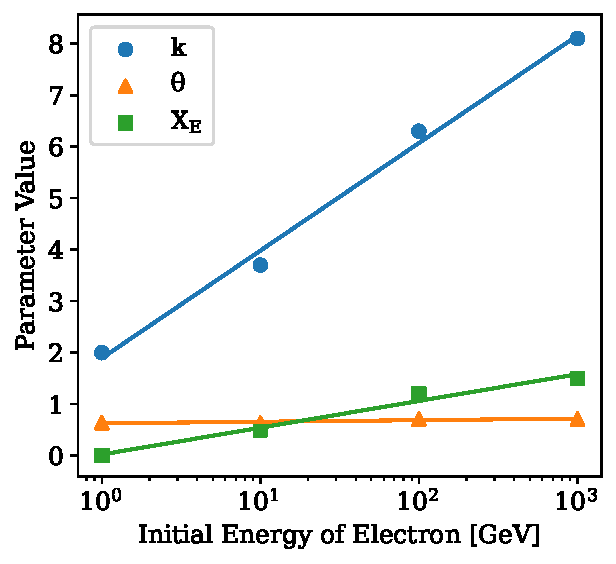
\includegraphics[width=0.6\linewidth]{img/param_X_parameter.pdf}
    \caption{电磁簇射中切伦科夫光子的纵向分布表达式中的参数随能量的变化。}
    \label{fig:param_X_parameter}
\end{figure}

电磁簇射中产生切伦科夫的次级粒子的运动方向与入射电子之间的夹角$\theta_p$的分布如图\ref{fig:param_costh_distribution}中所示,该分布不随入射电子能量的变化而变化,可以用如下公式来表示:
\begin{equation}
\begin{aligned}
  f(\hat{C}) &= \frac{\theta^k}{\Gamma(k)} \times \hat{C}^{k-1} * e^{-\hat{C} \theta}  \\
  \hat{C} &= 1 + C_s - \cos\theta ,
\end{aligned}
\end{equation}
其中$k=0.05$,$\theta=1.6$,$C_s=0.001$是拟合参数。

\begin{figure}[htb]
    \centering
    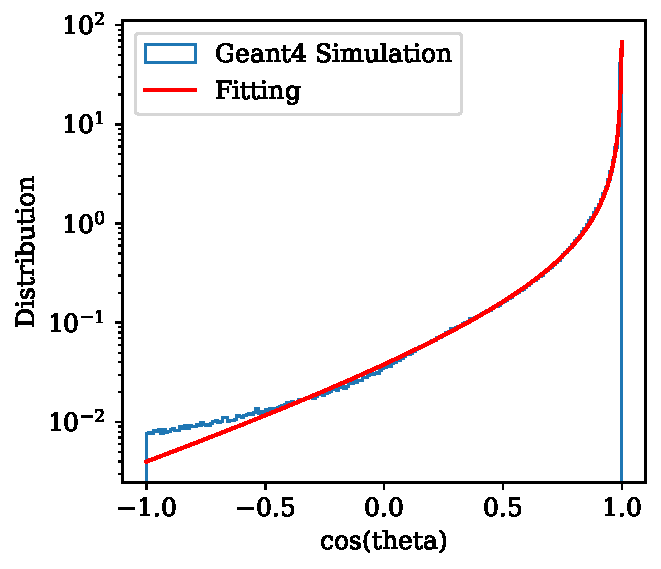
\includegraphics[width=0.6\linewidth]{img/param_costh_distribution.pdf}
    \caption{电磁簇射中次级粒子的运动方向与初始入射电子之间的夹角的分布。}
    \label{fig:param_costh_distribution}
\end{figure}

电磁簇射中产生的切伦科夫光子与簇射中心的纵向距离$R$上的分布的90\%百分位处的值$R_{90}$如图\ref{fig:param_r90}中所示,可以用如下参数化的表达式来近似:
\begin{equation}
    R_{90}(X) = ax^2 + bx + c ,
\end{equation}
其中$a=0.0012$,$b=0.0740$,$c=0.065$是二次多项式的拟合参数。

\begin{figure}[htb]
    \centering
    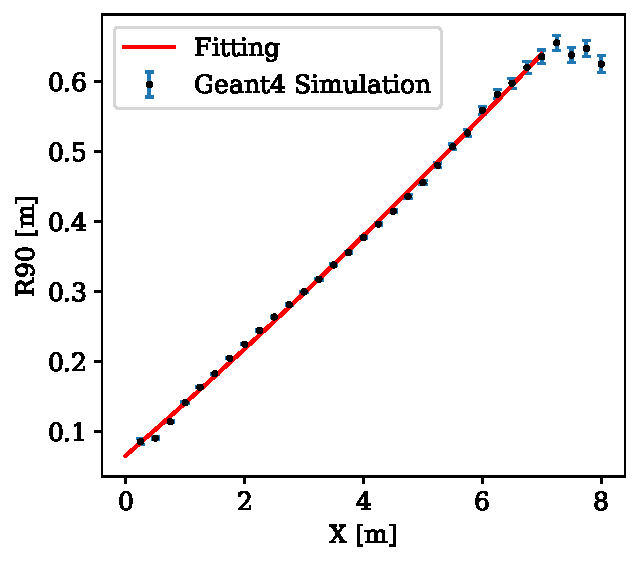
\includegraphics[width=0.6\linewidth]{img/param_r90.pdf}
    \caption{电磁簇射中切伦科夫光子的纵向分布表达式中的参数随能量的变化。}
    \label{fig:param_r90}
\end{figure}




% \lstinputlisting[language=C++]{code/DIS_example.cpp}
